\documentclass[]{ximera}
%handout:  for handout version with no solutions or instructor notes
%handout,instructornotes:  for instructor version with just problems and notes, no solutions
%noinstructornotes:  shows only problem and solutions

%% handout
%% space
%% newpage
%% numbers
%% nooutcomes

%I added the commands here so that I would't have to keep looking them up
%\newcommand{\RR}{\mathbb R}
%\renewcommand{\d}{\,d}
%\newcommand{\dd}[2][]{\frac{d #1}{d #2}}
%\renewcommand{\l}{\ell}
%\newcommand{\ddx}{\frac{d}{dx}}
%\everymath{\displaystyle}
%\newcommand{\dfn}{\textbf}
%\newcommand{\eval}[1]{\bigg[ #1 \bigg]}

%\begin{image}
%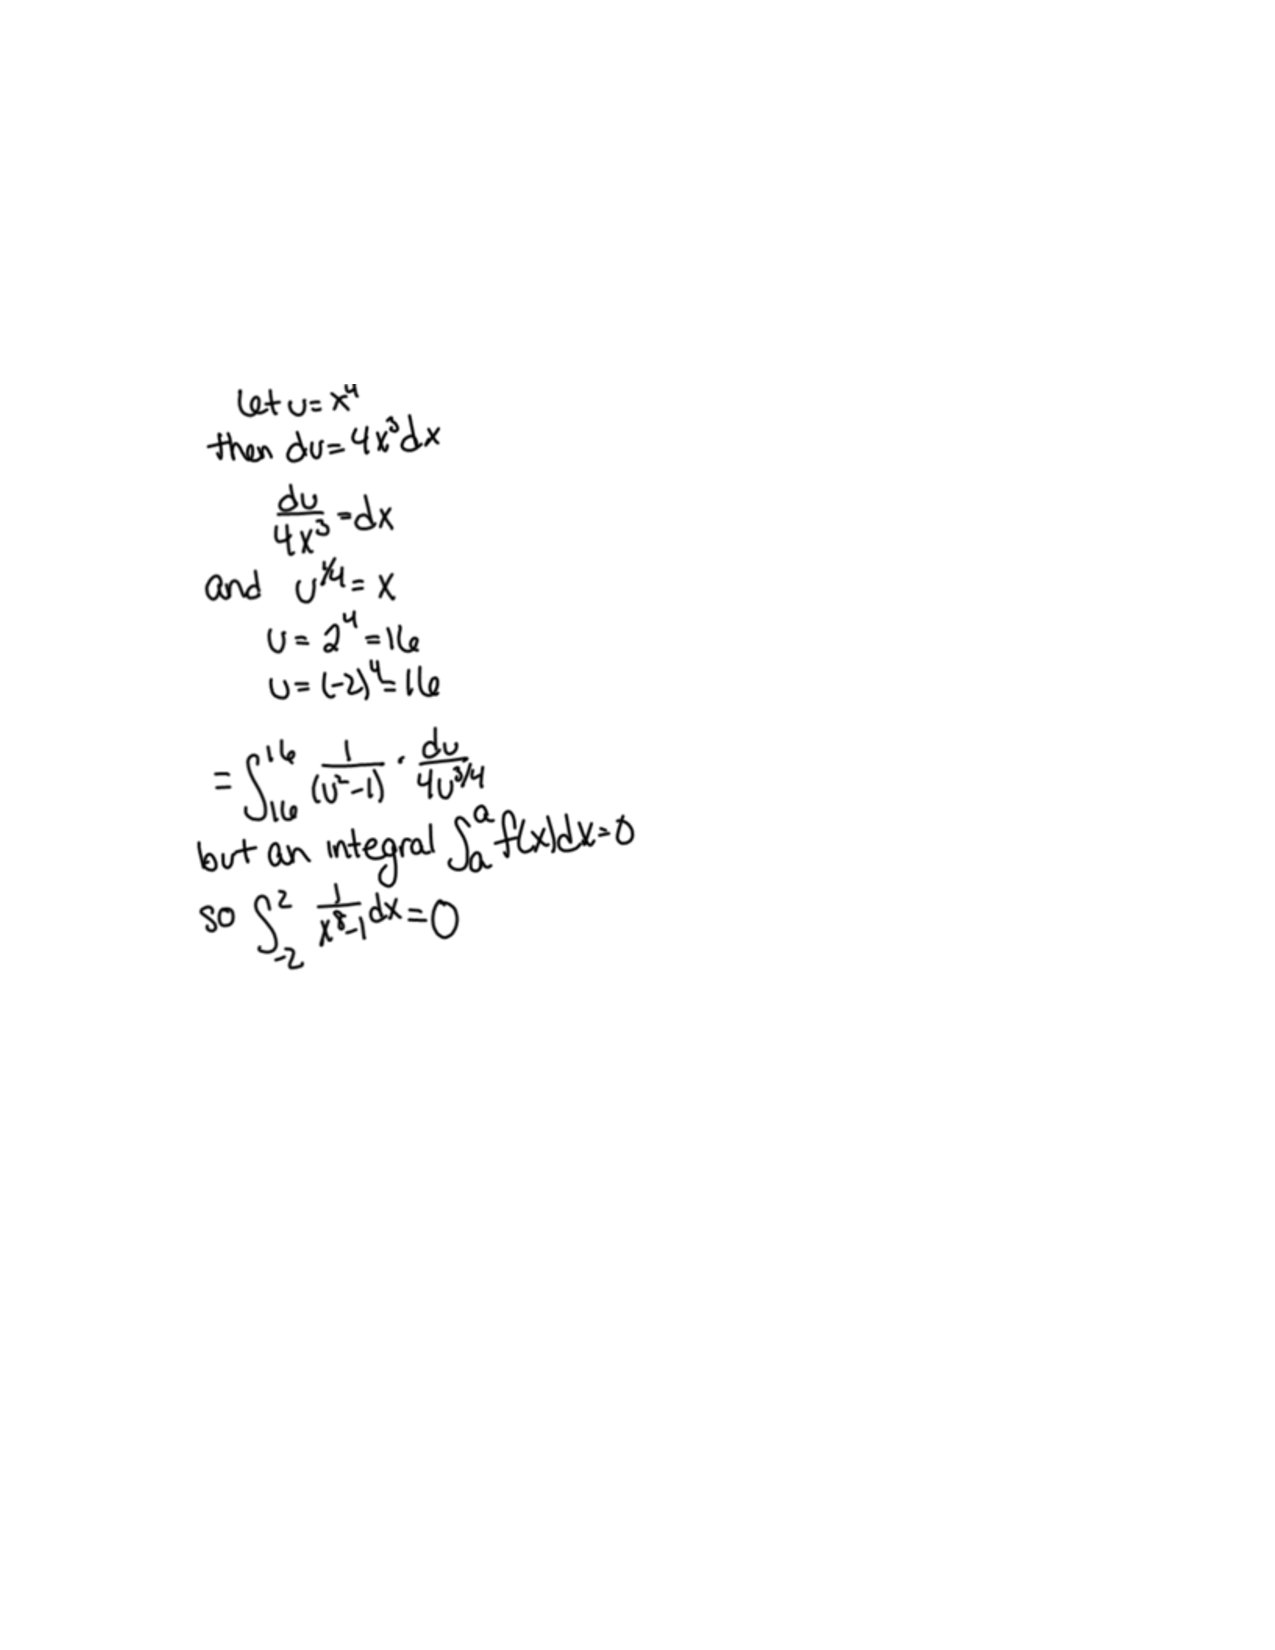
\includegraphics[trim= 170 420 250 180]{Figure1.pdf}
%\end{image}

%add a ``.'' below when used in a specific directory.
\newcommand{\RR}{\mathbb R}
\renewcommand{\d}{\,d}
\newcommand{\dd}[2][]{\frac{d #1}{d #2}}
\renewcommand{\l}{\ell}
\newcommand{\ddx}{\frac{d}{dx}}
\newcommand{\dfn}{\textbf}
\newcommand{\eval}[1]{\bigg[ #1 \bigg]}

\usepackage{multicol}

\renewenvironment{freeResponse}{
\ifhandout\setbox0\vbox\bgroup\else
\begin{trivlist}\item[\hskip \labelsep\bfseries Solution:\hspace{2ex}]
\fi}
{\ifhandout\egroup\else
\end{trivlist}
\fi} %% we can turn off input when making a master document

\title{Sequences}  

\begin{document}
\begin{abstract}		\end{abstract}
\maketitle



\begin{comment}
\section{Warm up:}

	\begin{freeResponse}
	
	\end{freeResponse}
	
\begin{instructorNotes}

\end{instructorNotes}
\end{comment}







\section{Group work:}



%problem 1
\begin{problem}
For each of the following sequences, find the limit as the number of terms approaches infinity.
	\begin{enumerate}
	
	\item  $a_n = \left( \frac{n+1}{2n} \right) \left( \frac{n-2}{n} \right)^{\frac{n}{2}}$
	\begin{freeResponse}
	Let $f(x) =  \left( \frac{x+1}{2x} \right) \left( \frac{x-2}{x} \right)^{\frac{x}{2}}$.  
	Then
		\begin{align*}
		\lim_{x \to \infty} f(x) 
		&= \lim_{x \to \infty} e^{\ln f(x)}  \\
		&= e^{\lim_{x \to \infty} \ln f(x)}.
		\end{align*}
	So we need to compute the limit in the exponent.  To this end
		\begin{align*}
		\lim_{x \to \infty} \ln f(x) 
		&= \lim_{x \to \infty} \left[ \ln \left( \frac{x+1}{2x} \right) + \ln \left( \frac{x-2}{x} \right)^{\frac{x}{2}} \right]  \\
		&= \lim_{x \to \infty} \ln \left( \frac{x+1}{2x} \right) + \lim_{x \to \infty} \left[ \frac{x}{2} \ln \left( \frac{x-2}{x} \right) \right]  \quad {\color{red}\text{provided both limits exist}}  \\
		&= \ln \left( \frac{1}{2} \right) + \lim_{x \to \infty} \frac{\ln \left( 1 - \frac{2}{x} \right)}{\frac{2}{x}}  \quad {\color{red}\text{indeterminant of the form }\frac{0}{0}}\\
		&= \ln \left( \frac{1}{2} \right) + \lim_{x \to \infty} \frac{\frac{2x^{-2}}{1-\frac{2}{x}}}{-2x^{-2}}  \quad {\color{red}\text{L'Hospital's Rule}}  \\
		&= \ln \left( \frac{1}{2} \right) + \lim_{x \to \infty} \frac{-1}{1-\frac{2}{x}}  \\
		&= \ln \left( \frac{1}{2} \right) - 1.
		\end{align*}
	So 
		\[
		\lim_{x \to \infty} f(x) = e^{\ln \left( \frac{1}{2} \right) - 1} = \frac{1}{2} e^{-1}
		\]
	and therefore
		\[
		\lim_{n \to \infty} \left( \frac{n+1}{2n} \right) \left( \frac{n-2}{n} \right)^{\frac{n}{2}} = \frac{1}{2} e^{-1}.
		\]
	\end{freeResponse}
	
	
	
	\item  $a_n = \sqrt[n]{3^{2n+1}}$
	\begin{freeResponse}
		\begin{align*}
		\lim_{n \to \infty} \sqrt[n]{3^{2n+1}}
		&= \lim_{n \to \infty} \left( 3^{2n+1} \right)^{\frac{1}{n}}  \\
		&= \lim_{n \to \infty} 3^{2 + \frac{1}{n}}  \\
		&= \lim_{n \to \infty} 3^2 \cdot 3^{\frac{1}{n}}  \\
		&= 9 \lim_{n \to \infty} e^{\frac{1}{n}}  \\
		&= 9 \cdot 3^0  \\
		&= 9 \cdot 1 = 9.
		\end{align*}
	\end{freeResponse}
	
	
	
	\item  $a_n = \left( \sqrt{n^2+7} - n \right)$
	\begin{freeResponse}
		\begin{align*}
		\lim_{n \to \infty} \left( \sqrt{n^2+7} - n \right)
		&= \lim_{n \to \infty} \left[ \left( \sqrt{n^2 + 7} - n \right) \cdot \frac{\sqrt{n^2 + 7} + n}{\sqrt{n^2 + 7} + n} \right]  \\
		&= \lim_{n \to \infty} \frac{n^2 + 7 - n^2}{n \sqrt{1 + \frac{7}{n^2}} + n}  \\
		&= \lim_{n \to \infty} \frac{7}{n ( \sqrt{1 + \frac{7}{n^2}} + 1)}  \\
		&= 0.
		\end{align*}
	\end{freeResponse}
	
	
	
	\item  $a_n = \frac{(2n+3)!}{5n^3 (2n)!}$
	\begin{freeResponse}
		\begin{align*}
		\lim_{n \to \infty} \frac{(2n+3)!}{5n^3(2n)!}
		&= \lim_{n \to \infty} \frac{(2n+3)(2n+2)(2n+1)(2n)!}{5n^3(2n)!}  \\
		&= \lim_{n \to \infty} \frac{(2n+3)(2n+2)(2n+1)}{5n^3}  \\
		&= \frac{8}{5} 	\quad	{\color{red}\text{Compare the coefficients of the leading }n^3 \text{terms}}
		\end{align*}
	\end{freeResponse}
	
	
	
	\item  $a_n = (2^n + 3^n)^{\frac{1}{n}}$  
	\begin{center}
	{\it Hint:  $a_n \geq (0+3^n)^{\frac{1}{n}} = 3$ and $a_n \leq (2 \cdot 3^n)^{\frac{1}{n}} = 2^{\frac{1}{n}} \cdot 3$}
	\end{center}
	\begin{freeResponse}
	From the hint
		\[
		3 = (0+3^n)^\frac{1}{n}  \leq a_n \leq (2 \cdot 3^n)^\frac{1}{n} = 2^\frac{1}{n} \cdot 3.
		\]
	So by the squeeze theorem, we have that
		\begin{align*}
		\lim_{n \to \infty} 3 \leq &\lim_{n \to \infty} a_n \leq \lim_{n \to \infty} 2^\frac{1}{n} \cdot 3  \\
		\Longrightarrow 	\qquad	3 \leq &\lim_{n \to \infty} a_n \leq 1 \cdot 3 = 3.
		\end{align*}
	Thus,
		\[
		\lim_{n \to \infty} a_n = 3.
		\]
	\end{freeResponse}
	
	
	
	\item  $a_n = \frac{n^{365} + 5^n}{8^n + n^3}$
	\begin{freeResponse}
		\begin{align*}
		\lim_{n \to \infty} \frac{n^{365} + 5^n}{8^n + n^3}
		&= \lim_{n \to \infty} \frac{n^{365} + 5^n}{8^n + n^3} \cdot \frac{\frac{1}{8^n}}{\frac{1}{8^n}}  \\
		&=  \lim_{n \to \infty} \frac{\frac{n^{365}}{8^n} + \left( \frac{5}{8} \right)^n}{1 + \frac{n^3}{8^n}}  \\
		&= \frac{0+0}{1+0} = 0.		\quad	{\color{red}\text{due to growth rates,} \lim_{n \to \infty} \frac{n^k}{a^n} = 0.}
		\end{align*}
	\end{freeResponse}
	
	
	
	\item  $a_n = \cos(n \pi)$
	\begin{freeResponse}
	\[
	\lim_{n \to \infty} \cos(n \pi) \text{ does not exist}.
	\]
	This is because $\cos(n \pi) = 1$ when $n$ is even, and $\cos(n \pi) = -1$ when $n$ is odd.
	\end{freeResponse}
	
	\end{enumerate}
	
\end{problem}

\begin{instructorNotes}
For this problem, give each group two of the problems to report on.  
Give about $8$ minutes (or less?) for the group work and about $10-15$ minutes for discussion.  
On (a), L'Hospital's Rule is involved.  
On (e), the squeeze theorem should be involved.  
On (f), the students may use ``known'' facts of the relative growth of polynomial vs. exponential terms.
\end{instructorNotes}







%problem 2
\begin{problem}
Show that 
$$\lim_{n \to \infty} \left( \sqrt{n+1} - \sqrt{n} \right)$$ 
exists by proving that $a_n = \sqrt{n+1} - \sqrt{n}$ is a bounded monotonic sequence.  A hint is to show that $f(x) = \sqrt{x+1} - \sqrt{x}$ is a decreasing function by showing that $f'(x) < 0$.  
	\begin{freeResponse}
	Let $f(x) = \sqrt{x+1} - \sqrt{x}$.  Then
		\begin{align*}
		f'(x) 
		&= \frac{1}{2 \sqrt{x+1}} - \frac{1}{2 \sqrt{x}}  \\
		&= \frac{\sqrt{x} - \sqrt{x+1}}{2 \sqrt{x}\sqrt{x+1}}  \\
		&< 0
		\end{align*}
	since the denominator is clearly positive, and $\sqrt{x} < \sqrt{x+1}$.
	Therefore $f$ is decreasing, and so the original sequence is decreasing.  
	Also notice that since 
	$$\sqrt{x} < \sqrt{x+1}$$
	we have that 
	$$0 < \sqrt{x+1} - \sqrt{x} = f(x).$$
	Thus the original sequence is bounded below by $0$.  \

	Therefore, since the sequence $\left\{ \sqrt{n+1} - \sqrt{n} \right\}$ is bounded and monotone decreasing, the limit
		\[
		\lim_{n \to \infty} \sqrt{n+1} - \sqrt{n}
		\]
	exists.
	\end{freeResponse}
		
\end{problem}

\begin{instructorNotes}
Perhaps do as a whole class discussion.  
Emphasize careful writing of reasoning.
\end{instructorNotes}







%problem 3
\begin{problem}
Find the limit of the given sequence.  
Also, determine if it is a geometric sequence.
	\begin{multicols}{3}
	\begin{enumerate}
	
	\item  $a_n = \frac{n^2}{2^n}$
	%\begin{freeResponse}
	
	%\end{freeResponse}
	
	
	
	\item  $a_n = \frac{1}{3^n}$
	%\begin{freeResponse}
	
	%\end{freeResponse}
	
	
	
	\item  $a_n = \left( \frac{1}{n} \right)^4$
	%\begin{freeResponse}
	
	%\end{freeResponse}
	
	
	
	\item  $a_n = \frac{e^n + (-3)^n}{5^n}$
	%\begin{freeResponse}
	
	%\end{freeResponse}
	
	
	
	\item  $a_n = 3^{\frac{1}{n}}$
	%\begin{freeResponse}
	
	%\end{freeResponse}
	
	\end{enumerate}
	\end{multicols}
	
	\begin{freeResponse}
	\begin{enumerate}
	\item 	$\lim_{n \to \infty} \frac{n^2}{2^n} = 0 	\quad	{\color{red}\text{growth rate}}$
	
	\item  $\lim_{n \to \infty} \frac{1}{3^n} = \lim_{n \to \infty} \left( \frac{1}{3} \right)^n = 0.$
	This is a geometric sequence with $a = 1$ and $r = \frac{1}{3}$.  
	
	\item  $\lim_{n \to \infty} \left( \frac{1}{n} \right)^4 = 0$.  
	
	\item  $\lim_{n \to \infty} \frac{e^n + (-3)^n}{5^n} = \lim_{n \to \infty} \left[ \left( \frac{e}{5} \right)^n + \left( \frac{-3}{5} \right)^n \right] = 0.$  
	
	This is the sum of two geometric sequences.  
	For both, the initial term is $a = 1$.  
	For the first sequence the ratio is $r_1 = \frac{e}{5}$, and for the second the ratio is $r_2 = \frac{-3}{5}$.
	
	\item  $\lim_{n \to \infty} 3^\frac{1}{n} = 3^0 = 1$.  
	
	\end{enumerate}
	\end{freeResponse}

\end{problem}

\begin{instructorNotes}
These limits should be relatively easy to analyze.  
The students need to identify the ``$r$'' if it is a geometric sequence (and note that the exponent $n$ is the variable).  
On (d) and (f), they should argue that they are looking at the sum of two geometric sequences.  
Maybe give one per group with about $8$ minutes for discussion.  
\end{instructorNotes}
















	
	
	
	
	
	
	
	
	

	










								
				
				
	














\end{document} 


















